
\section{Στοιχεία}


% ------------------------------------------------------------------------------------------
% ΜΕΛΕΤΗ ΟΠΤΙΚΩΝ ΔΙΑΚΟΠΤΩΝ ΠΥΡΙΤΙΟΥ (Si) ΓΙΑ ΤΗ ΔΡΟΜΟΛΟΓΗΣΗ ΠΛΗΡΟΦΟΡΙΑΣ ΣΕ ΥΠΟΛΟΓΙΣΤΙΚΑ ΚΕΝΤΡΑ
% ------------------------------------------------------------------------------------------

Πριν παρουσιάσουμε κάποια ερευνητικά προγράμματα θα αναφερθούμε 
συνοπτικά στους βασικούς τύπους οπτικών διακοπτών και στους τρόπους 
λειτουργίας των τεχνολογιών τους. 
Η επιστράτευση της Φωτονικής Τεχνολογίας Πυριτίου (Silicon Photonics
Technology) για την ενσωμάτωση των διάφορων οπτικών εξαρτημάτων σε
κοινό υπόστρωμα υπόσχεται τη μαζική παραγωγή σύνθετων διατάξεων
χαμηλού κόστους.

\subsection{Μηχανικοί Διακόπτες}

Στους διακόπτες αυτούς η εναλλαγή πραγματοποιείται από μηχανικά
μέσα. Ένα είδος τέτοιου διακόπτη χρησιμοποιεί μια διαρρύθμιση
διακοπτών όπου η κατάσταση εναλλαγής καθορίζεται από τη μετακίνηση
ενός καθρέφτη μέσα και έξω από το οπτικό μονοπάτι. Άλλο είδος διακόπτη
μπορεί να χρησιμοποιεί κατευθυνόμενο συζευκτήρα κυκλωμάτων
(directional coupler). Τεντώνοντας ή λυγίζοντας την ίνα στην περιοχή
αλληλεπίδρασης, αλλάζει ο λόγος σύζευξης του συζευκτήρα και κατά
συνέπεια μπορούμε να τον χρησιμοποιήσουμε για να εκτρέψουμε το φως από
μία θύρα εισόδου σε διαφορετικές θύρες εξόδου. Οι διακόπτες αυτοί
έχουν μικρή απώλεια εισόδου, μικρό PDL, χαμηλό crosstalk και είναι
σχετικά φτηνοί. Έχουν όμως ταχύτητες εναλλαγής της τάξης μερικών ms
και για αυτό το λόγο χρησιμοποιούνται μόνο στην περίπτωση της διάθεσης
των φωτεινών μονοπατιών.

\subsection{Θερμο-Οπτικοί Διακόπτες}

Πρόκειται για 2x2 συνδυασμένους μετρητές παρεμβολών (interferometers),
οι οποίοι κατασκευάζονται σε κυματοδηγά υλικά, που κατασκευάζονται από
πολυμερή ή σιλικόνη, των οποίων ο δείκτης διάθλασης είναι συνάρτηση
της θερμοκρασίας. Αλλάζοντας τον δείκτη διάθλασης στον έναν βραχίονα
του interferometer, η σχετική διαφορά φάσης μεταξύ των δύο βραχιόνων
αλλάζει, έχοντας ως αποτέλεσμα την καθοδήγηση του σήματος εισόδου από
μία θύρα εξόδου σε άλλη.  Οι συσκευές αυτές κατασκευάζονται από
πυρίτιο όπως και από πολυμερή του, αλλά έχουν πολύ χαμηλό
crosstalk. Επίσης, το θέρμο-οπτικό φαινόμενο είναι πολύ αργό και οι
ταχύτητες εναλλαγής είναι της τάξης των μερικών ms. Η βραδύτητα τους
δεν τους περιορίζει στις ήδη υπάρχουσες εφαρμογές.

\subsection{Ηλεκτρο-Οπτικοί Διακόπτες}

Ένας τέτοιος 2x2 διακόπτης επιλέγει τις διαδρομές των φωτεινών κυμάτων
μέσα σε ενεργές συσκευές χρησιμοποιώντας πολωμένο ηλεκτρικό
ρεύμα. Χρησιμοποιούν έναν κατευθυνόμενο συζευκτήρα (directional
coupler), του οποίου η αναλογία σύζευξης τροποποιείται με την αλλαγή
του δείκτη διάθλασης του υλικού που βρίσκεται στην περιοχή
σύζευξης. Το υλικό που χρησιμοποιείται είναι το Lithium
Niobate-LiNbO3. Η εναλλαγή πραγματοποιείται με την εφαρμογή κατάλληλης
τάσης στα ηλεκτρόδια.

Ένας τέτοιος διακόπτης μπορεί να αλλάζει κατάσταση πολύ γρήγορα
συνήθως σε λιγότερο από 1 ns. Ο χρόνος αυτός καθορίζεται από τη
δυναμικότητα των ηλεκτροδίων. Λόγω της ιδιότητας αυτής, ένας τέτοιος
διακόπτης χρησιμοποιείται συχνά ως εξωτερικός διαμορφωτή \cite{conta}. Οι
διακόπτες αυτοί έχουν συνήθως μεγάλη απώλεια και PDL και είναι πιο
ακριβοί από τους μηχανικούς. Εντούτοις, ούτε τα ήλεκτρο-οπτικά αλλά
ούτε και τα θερμό-οπτικά switches δεν μπορούν ακόμα να επιτύχουν την
απώλεια εισαγωγής, το back reflection και τη long-term σταθερότητα των
οπτό-μηχανικών οπτικών switches.

\subsection{Ημιαγωγικοί Διακόπτες Οπτικών Ενισχυτών}

Πρόκειται για on-off διακόπτες που χρησιμοποιούν τον Semiconductor
Optical Amplifier (SOA). Λειτουργούν με αλλαγή της διαφοράς δυναμικού,
aν η διαφορά δυναμικού μειωθεί, δεν γίνεται αναστροφή πληθυσμού
(population inversion) και η συσκευή απορροφά τα εισερχόμενα σήματα. Ο
συνδυασμός της ενίσχυσης στην κατάσταση on και της απορρόφησης στην
off μεγαλώνει πάρα πολύ το λόγο εξασθένισης του σήματος εντός της
συσκευής. Η ταχύτητα εναλλαγής είναι 1 ns. Το υλικό από το οποίο
αποτελούνται είναι ακριβό και πολύ δύσκολο να είναι ανεξάρτητο της
πόλωσης.

\subsection{Οπτικός Συμβολομετρικός Διακόπτης}

Για πρώτη φορά, η χρήση συμβολόμετρων για την υλοποίηση αμιγώς οπτικών
διακοπτών προτάθηκε στις αρχές της δεκαετίας του 1980 \cite{1071766}
και είναι ευρέως αποδεκτό πλέον ότι οι οπτικές συμβολομετρικές
διατάξεις μπορούν να προσφέρουν πλεονεκτήματα στην ταχύτητα
λειτουργίας, στη δυνατότητα υλοποίησης Boolean λογικής, καθώς και σε
ένα ευρύτερο φάσμα εφαρμογών \cite{Patel:98}.  Για την επιτυχή
λειτουργία του συμβολόμετρου απαιτείται η ύπαρξη δύο τουλάχιστον
οπτικών σημάτων. Το ένα από τα δύο σήματα εισέρχεται στο διακόπτη σαν
σήμα εισόδου και το δεύτερο οπτικό σήμα, που απαιτείται, είναι το σήμα
ελέγχου (control signal), το οποίο μπορεί να είναι μια τυχαία παλμική
ακολουθία, και του οποίου ο ρόλος είναι να καθορίζει-ελέγχει την
κατάσταση μεταγωγής του διακόπτη.

Το σήμα εισόδου διαχωρίζεται, καθώς εισέρχεται στη διάταξη, σε δύο
συνιστώσες με τη βοήθεια ενός οπτικού συζεύκτη ισχύος. Στη συνέχεια, η
κάθε μια συνιστώσα διαδίδεται στον ένα από τους δύο βραχίονες του
συμβολόμετρου και τελικά οι δύο συνιστώσες επανενώνονται στην έξοδο,
μέσω ενός δεύτερου οπτικού συζεύκτη ισχύος. Το μέγεθος της οπτικής
ισχύος σε κάθε έξοδο της πύλης είναι συνάρτηση της συμβολής των δύο
συνιστωσών. Αν τα υλικά, που αποτελούν τους δύο βραχίονες ιδίου
μήκους, έχουν τα ίδια χαρακτηριστικά, τότε οι αντίστοιχοι οπτικοί
δρόμοι είναι ίδιοι και οι δύο συνιστώσες του σήματος ρολογιού έχουν
την ίδια φάση (phase), όταν συμβάλλουν στο δεύτερο
συζεύκτη. Αποτέλεσμα αυτού είναι στη μια έξοδο του διακόπτη να υπάρχει
πλήρως προσθετική συμβολή, ενώ στην άλλη έξοδο του διακόπτη η συμβολή
να είναι πλήρως αναιρετική. Κατά συνέπεια, το σύνολο της οπτικής
ισχύος εξέρχεται, σ’ αυτήν την περίπτωση, από την πρώτη θύρα εξόδου
και ο διακόπτης βρίσκεται στην κατάσταση OFF.

\begin{figure}[H]
  \centering
  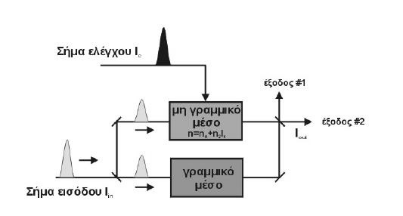
\includegraphics[width=.7\linewidth]{interf.png}
  \caption{Σχηματική παράσταση συμβολομέτρων Mach-Zehnder}
  \label{fig:mzi}
\end{figure}


Η διέγερση της μη γραμμικότητας του μέσου επιτυγχάνεται με την
εισαγωγή ενός ισχυρού οπτικού σήματος ελέγχου και η προκαλούμενη
μεταβολή του δείκτη διάθλασης του μη γραμμικού μέσου γίνεται αντιληπτή
από το ασθενούς ισχύος σήμα εισόδου, ως μια αλλαγή στη φάση
του. Αποτέλεσμα αυτού, είναι να φτάνουν οι δύο συνιστώσες του σήματος
εισόδου στην έξοδο με διαφορετική μεταξύ τους φάση, οπότε η συμβολή
τους μετατρέπει τη διαφορά φάσης σε μεταβολή πλάτους, αλλάζοντας το
συσχετισμό οπτικής ισχύος στις δύο θύρες εξόδου του διακόπτη. Στην
περίπτωση που η μεταβολή στη φάση είναι ίση με π, το σύνολο της
οπτικής ισχύος εξέρχεται από τη δεύτερη θύρα του διακόπτη, πλέον, και
όχι από την πρώτη, και η πύλη είναι σε κατάσταση μεταγωγής ή ON.

\subsection{Συμβολόμετρο Mach-Zehnder (MZI)}


Tα συμβολόμετρα Mach-Zehnder (Mach-Zehnder Interferometer (ΜΖΙ)) είναι
γενικά οπτικές συσκευές που βασίζονται στο φαινόμενο της
συμβολής. Τυπικά ενεργοποιούνται με κάποιο σήμα εισόδου ενώ στη
συνέχεια χωρίζουν το σήμα αυτό σε δύο υποσήματα χρησιμοποιώντας κάποιο
διαχωριστή (συνήθως κάτοπτρα μερικής εκπομπής), και εν συνεχεία
υποβάλλοντας την ακτίνα σε κάποιες εξωτερικές επιδράσεις, (πχ. αλλαγή
μήκους κύματος ή χρονική ολίσθηση) και τελικά ενώνοντας τα δύο
υποσήματα σε ένα μοναδικό. Λειτουργεί με συμβολή διαίρεσης πλάτους.
Όπως φαίνεται και στην Εικόνα \ref{fig:mzi}  χρησιμοποιεί δύο διαφορετικούς
διαχωριστές σήματος για να διαχωρίσει και να συνδυάσει τα σήματα, και
έχει δύο εξόδους που μπορεί να συνδέονται σε φωτοανιχνευτές ή άλλες
διατάξεις.

\begin{figure}[H]
  \centering
  \includegraphics[width=.7\linewidth]{mzi.png}
  \caption{Σχηματική παράσταση συμβολομέτρων Mach-Zehnder}
  \label{fig:mzi}
\end{figure}

Αν το συμβολόμετρο είναι καλά ευθυγραμμισμένο η διαφορά των μηκών των
κλάδων του μπορεί να προσαρμοστεί (πχ. κινώντας ένα από τα κάτοπτρα ή
τοποθετώντας διαφορετικού μήκους ίνα) με τέτοιο τρόπο ώστε για
συγκεκριμένη οπτική συχνότητα το σύνολο της ισχύος να εξάγεται σε μία
μόνο έξοδο.

\subsection{Σύνοψη}

Αυτοί οι τύποι διακοπτών είναι
απαραίτητα στοιχεία των οπτικών δρομολογητών και αποτελούν δομικούς 
λίθους στη συναρμογή των αρχιτεκτονικών ερευνητικών προγραμμάτων
που θα εξεταστούν στη συνέχεια.

%%% Local Variables:
%%% mode: latex
%%% TeX-master: "main"
%%% TeX-engine: xetex
%%% End:
